% Created by tikzDevice version 0.10.1 on 2017-04-10 15:24:32
% !TEX encoding = UTF-8 Unicode
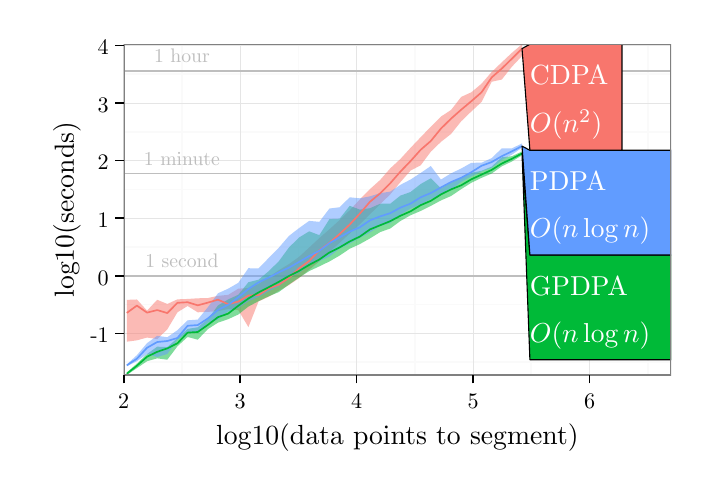
\begin{tikzpicture}[x=1pt,y=1pt]
\definecolor{fillColor}{RGB}{255,255,255}
\path[use as bounding box,fill=fillColor,fill opacity=0.00] (0,0) rectangle (238.49,158.99);
\begin{scope}
\path[clip] (  0.00,  0.00) rectangle (238.49,158.99);
\definecolor{drawColor}{RGB}{255,255,255}
\definecolor{fillColor}{RGB}{255,255,255}

\path[draw=drawColor,line width= 0.6pt,line join=round,line cap=round,fill=fillColor] (  0.00,  0.00) rectangle (238.49,158.99);
\end{scope}
\begin{scope}
\path[clip] ( 34.70, 33.48) rectangle (232.49,152.99);
\definecolor{fillColor}{RGB}{255,255,255}

\path[fill=fillColor] ( 34.70, 33.48) rectangle (232.49,152.99);
\definecolor{drawColor}{gray}{0.98}

\path[draw=drawColor,line width= 0.6pt,line join=round] ( 34.70, 38.08) --
	(232.49, 38.08);

\path[draw=drawColor,line width= 0.6pt,line join=round] ( 34.70, 58.90) --
	(232.49, 58.90);

\path[draw=drawColor,line width= 0.6pt,line join=round] ( 34.70, 79.72) --
	(232.49, 79.72);

\path[draw=drawColor,line width= 0.6pt,line join=round] ( 34.70,100.54) --
	(232.49,100.54);

\path[draw=drawColor,line width= 0.6pt,line join=round] ( 34.70,121.35) --
	(232.49,121.35);

\path[draw=drawColor,line width= 0.6pt,line join=round] ( 34.70,142.17) --
	(232.49,142.17);

\path[draw=drawColor,line width= 0.6pt,line join=round] ( 55.74, 33.48) --
	( 55.74,152.99);

\path[draw=drawColor,line width= 0.6pt,line join=round] ( 97.82, 33.48) --
	( 97.82,152.99);

\path[draw=drawColor,line width= 0.6pt,line join=round] (139.91, 33.48) --
	(139.91,152.99);

\path[draw=drawColor,line width= 0.6pt,line join=round] (181.99, 33.48) --
	(181.99,152.99);

\path[draw=drawColor,line width= 0.6pt,line join=round] (224.07, 33.48) --
	(224.07,152.99);
\definecolor{drawColor}{gray}{0.90}

\path[draw=drawColor,line width= 0.2pt,line join=round] ( 34.70, 48.49) --
	(232.49, 48.49);

\path[draw=drawColor,line width= 0.2pt,line join=round] ( 34.70, 69.31) --
	(232.49, 69.31);

\path[draw=drawColor,line width= 0.2pt,line join=round] ( 34.70, 90.13) --
	(232.49, 90.13);

\path[draw=drawColor,line width= 0.2pt,line join=round] ( 34.70,110.95) --
	(232.49,110.95);

\path[draw=drawColor,line width= 0.2pt,line join=round] ( 34.70,131.76) --
	(232.49,131.76);

\path[draw=drawColor,line width= 0.2pt,line join=round] ( 34.70,152.58) --
	(232.49,152.58);

\path[draw=drawColor,line width= 0.2pt,line join=round] ( 34.70, 33.48) --
	( 34.70,152.99);

\path[draw=drawColor,line width= 0.2pt,line join=round] ( 76.78, 33.48) --
	( 76.78,152.99);

\path[draw=drawColor,line width= 0.2pt,line join=round] (118.86, 33.48) --
	(118.86,152.99);

\path[draw=drawColor,line width= 0.2pt,line join=round] (160.95, 33.48) --
	(160.95,152.99);

\path[draw=drawColor,line width= 0.2pt,line join=round] (203.03, 33.48) --
	(203.03,152.99);
\definecolor{drawColor}{RGB}{190,190,190}

\path[draw=drawColor,line width= 0.6pt,line join=round] ( 34.70, 69.31) -- (232.49, 69.31);

\path[draw=drawColor,line width= 0.6pt,line join=round] ( 34.70,106.33) -- (232.49,106.33);

\path[draw=drawColor,line width= 0.6pt,line join=round] ( 34.70,143.35) -- (232.49,143.35);
\definecolor{fillColor}{RGB}{248,118,109}

\path[fill=fillColor,fill opacity=0.50] ( 35.81, 60.63) --
	( 39.47, 60.77) --
	( 43.14, 56.74) --
	( 46.80, 60.66) --
	( 50.46, 59.15) --
	( 54.12, 60.82) --
	( 57.79, 60.96) --
	( 61.45, 61.20) --
	( 65.11, 61.29) --
	( 68.77, 62.09) --
	( 72.43, 62.43) --
	( 76.10, 64.66) --
	( 79.76, 64.93) --
	( 83.42, 66.35) --
	( 87.08, 68.79) --
	( 90.74, 71.36) --
	( 94.41, 73.55) --
	( 98.07, 76.19) --
	(101.73, 79.55) --
	(105.39, 82.96) --
	(109.05, 86.14) --
	(112.72, 89.48) --
	(116.38, 93.00) --
	(120.04, 96.94) --
	(123.70,100.66) --
	(127.36,103.95) --
	(131.03,108.15) --
	(134.69,111.55) --
	(138.35,115.56) --
	(142.01,119.40) --
	(145.67,123.19) --
	(149.34,126.86) --
	(153.00,129.26) --
	(156.66,133.97) --
	(160.32,135.64) --
	(163.99,138.73) --
	(167.65,142.96) --
	(171.31,146.46) --
	(174.97,149.90) --
	(178.63,152.99) --
	(178.63,148.76) --
	(174.97,144.88) --
	(171.31,140.24) --
	(167.65,139.45) --
	(163.99,132.13) --
	(160.32,128.72) --
	(156.66,125.17) --
	(153.00,120.59) --
	(149.34,117.73) --
	(145.67,114.18) --
	(142.01,109.26) --
	(138.35,107.34) --
	(134.69,103.18) --
	(131.03, 98.79) --
	(127.36, 95.18) --
	(123.70, 91.59) --
	(120.04, 87.97) --
	(116.38, 84.59) --
	(112.72, 81.23) --
	(109.05, 78.00) --
	(105.39, 74.57) --
	(101.73, 71.54) --
	( 98.07, 68.49) --
	( 94.41, 65.98) --
	( 90.74, 63.90) --
	( 87.08, 61.74) --
	( 83.42, 60.07) --
	( 79.76, 50.79) --
	( 76.10, 56.95) --
	( 72.43, 57.30) --
	( 68.77, 56.56) --
	( 65.11, 56.29) --
	( 61.45, 56.14) --
	( 57.79, 58.42) --
	( 54.12, 56.14) --
	( 50.46, 49.99) --
	( 46.80, 46.47) --
	( 43.14, 47.02) --
	( 39.47, 46.01) --
	( 35.81, 45.52) --
	cycle;
\definecolor{fillColor}{RGB}{0,186,56}

\path[fill=fillColor,fill opacity=0.50] ( 35.81, 34.38) --
	( 39.47, 37.61) --
	( 43.14, 41.07) --
	( 46.80, 43.72) --
	( 50.46, 43.57) --
	( 54.12, 46.81) --
	( 57.79, 50.14) --
	( 61.45, 50.72) --
	( 65.11, 53.65) --
	( 68.77, 58.63) --
	( 72.43, 60.77) --
	( 76.10, 62.48) --
	( 79.76, 67.01) --
	( 83.42, 67.92) --
	( 87.08, 70.98) --
	( 90.74, 74.57) --
	( 94.41, 79.55) --
	( 98.07, 83.17) --
	(101.73, 85.39) --
	(105.39, 84.02) --
	(109.05, 89.81) --
	(112.72, 89.96) --
	(116.38, 94.61) --
	(120.04, 93.25) --
	(123.70, 93.76) --
	(127.36, 95.36) --
	(131.03, 95.39) --
	(134.69, 98.31) --
	(138.35, 99.61) --
	(142.01,102.49) --
	(145.67,104.56) --
	(149.34,100.96) --
	(153.00,103.02) --
	(156.66,104.90) --
	(160.32,106.54) --
	(163.99,107.27) --
	(167.65,108.78) --
	(171.31,112.15) --
	(174.97,112.55) --
	(178.63,114.25) --
	(178.63,112.86) --
	(174.97,110.64) --
	(171.31,108.88) --
	(167.65,106.27) --
	(163.99,104.72) --
	(160.32,102.94) --
	(156.66,100.64) --
	(153.00, 98.16) --
	(149.34, 96.57) --
	(145.67, 94.58) --
	(142.01, 92.76) --
	(138.35, 91.20) --
	(134.69, 89.13) --
	(131.03, 86.43) --
	(127.36, 85.11) --
	(123.70, 82.85) --
	(120.04, 80.79) --
	(116.38, 79.11) --
	(112.72, 76.64) --
	(109.05, 74.52) --
	(105.39, 72.74) --
	(101.73, 71.04) --
	( 98.07, 68.68) --
	( 94.41, 66.17) --
	( 90.74, 63.45) --
	( 87.08, 61.91) --
	( 83.42, 60.15) --
	( 79.76, 58.21) --
	( 76.10, 55.33) --
	( 72.43, 53.65) --
	( 68.77, 52.40) --
	( 65.11, 50.06) --
	( 61.45, 46.25) --
	( 57.79, 47.23) --
	( 54.12, 43.87) --
	( 50.46, 39.00) --
	( 46.80, 39.50) --
	( 43.14, 38.47) --
	( 39.47, 35.96) --
	( 35.81, 33.48) --
	cycle;
\definecolor{fillColor}{RGB}{97,156,255}

\path[fill=fillColor,fill opacity=0.50] ( 35.81, 37.30) --
	( 39.47, 40.65) --
	( 43.14, 45.00) --
	( 46.80, 47.64) --
	( 50.46, 47.13) --
	( 54.12, 49.68) --
	( 57.79, 53.24) --
	( 61.45, 53.50) --
	( 65.11, 57.96) --
	( 68.77, 63.01) --
	( 72.43, 64.66) --
	( 76.10, 66.78) --
	( 79.76, 72.07) --
	( 83.42, 71.98) --
	( 87.08, 75.75) --
	( 90.74, 79.47) --
	( 94.41, 83.73) --
	( 98.07, 86.57) --
	(101.73, 89.17) --
	(105.39, 88.83) --
	(109.05, 93.64) --
	(112.72, 94.10) --
	(116.38, 97.69) --
	(120.04, 97.33) --
	(123.70, 98.04) --
	(127.36, 99.19) --
	(131.03, 99.74) --
	(134.69,102.20) --
	(138.35,104.11) --
	(142.01,106.48) --
	(145.67,109.00) --
	(149.34,104.10) --
	(153.00,106.36) --
	(156.66,108.10) --
	(160.32,110.17) --
	(163.99,110.19) --
	(167.65,111.85) --
	(171.31,115.36) --
	(174.97,115.38) --
	(178.63,117.15) --
	(178.63,115.62) --
	(174.97,113.09) --
	(171.31,111.18) --
	(167.65,108.32) --
	(163.99,107.09) --
	(160.32,105.24) --
	(156.66,103.28) --
	(153.00,100.42) --
	(149.34, 98.58) --
	(145.67, 97.03) --
	(142.01, 95.06) --
	(138.35, 93.61) --
	(134.69, 91.39) --
	(131.03, 88.41) --
	(127.36, 87.36) --
	(123.70, 85.02) --
	(120.04, 83.06) --
	(116.38, 80.98) --
	(112.72, 79.19) --
	(109.05, 76.30) --
	(105.39, 74.63) --
	(101.73, 73.19) --
	( 98.07, 70.40) --
	( 94.41, 68.58) --
	( 90.74, 65.48) --
	( 87.08, 63.70) --
	( 83.42, 61.68) --
	( 79.76, 60.12) --
	( 76.10, 57.67) --
	( 72.43, 56.44) --
	( 68.77, 53.50) --
	( 65.11, 52.40) --
	( 61.45, 48.67) --
	( 57.79, 48.76) --
	( 54.12, 46.25) --
	( 50.46, 41.07) --
	( 46.80, 39.98) --
	( 43.14, 41.07) --
	( 39.47, 38.47) --
	( 35.81, 36.65) --
	cycle;
\definecolor{drawColor}{RGB}{248,118,109}

\path[draw=drawColor,line width= 0.6pt,line join=round] ( 35.81, 55.92) --
	( 39.47, 58.56) --
	( 43.14, 56.02) --
	( 46.80, 56.95) --
	( 50.46, 55.86) --
	( 54.12, 59.56) --
	( 57.79, 59.78) --
	( 61.45, 58.66) --
	( 65.11, 59.64) --
	( 68.77, 60.70) --
	( 72.43, 59.08) --
	( 76.10, 60.00) --
	( 79.76, 62.23) --
	( 83.42, 62.34) --
	( 87.08, 64.77) --
	( 90.74, 66.10) --
	( 94.41, 68.57) --
	( 98.07, 72.03) --
	(101.73, 74.70) --
	(105.39, 78.55) --
	(109.05, 81.28) --
	(112.72, 84.42) --
	(116.38, 87.87) --
	(120.04, 91.82) --
	(123.70, 96.09) --
	(127.36, 99.12) --
	(131.03,102.79) --
	(134.69,106.98) --
	(138.35,110.78) --
	(142.01,114.87) --
	(145.67,118.03) --
	(149.34,122.53) --
	(153.00,126.12) --
	(156.66,129.36) --
	(160.32,132.42) --
	(163.99,135.62) --
	(167.65,140.99) --
	(171.31,144.21) --
	(174.97,147.77) --
	(178.63,151.44);
\definecolor{drawColor}{RGB}{0,186,56}

\path[draw=drawColor,line width= 0.6pt,line join=round] ( 35.81, 33.94) --
	( 39.47, 36.82) --
	( 43.14, 40.09) --
	( 46.80, 41.86) --
	( 50.46, 43.09) --
	( 54.12, 44.94) --
	( 57.79, 48.80) --
	( 61.45, 49.02) --
	( 65.11, 51.60) --
	( 68.77, 54.39) --
	( 72.43, 55.66) --
	( 76.10, 58.50) --
	( 79.76, 61.12) --
	( 83.42, 63.32) --
	( 87.08, 65.20) --
	( 90.74, 67.14) --
	( 94.41, 69.26) --
	( 98.07, 71.09) --
	(101.73, 73.28) --
	(105.39, 75.21) --
	(109.05, 77.76) --
	(112.72, 79.58) --
	(116.38, 81.75) --
	(120.04, 83.51) --
	(123.70, 86.10) --
	(127.36, 87.59) --
	(131.03, 89.07) --
	(134.69, 91.02) --
	(138.35, 92.63) --
	(142.01, 94.85) --
	(145.67, 96.42) --
	(149.34, 98.73) --
	(153.00,100.55) --
	(156.66,102.04) --
	(160.32,104.21) --
	(163.99,105.89) --
	(167.65,107.59) --
	(171.31,109.89) --
	(174.97,111.61) --
	(178.63,113.54);
\definecolor{drawColor}{RGB}{97,156,255}

\path[draw=drawColor,line width= 0.6pt,line join=round] ( 35.81, 36.98) --
	( 39.47, 39.38) --
	( 43.14, 43.33) --
	( 46.80, 45.39) --
	( 50.46, 45.77) --
	( 54.12, 46.86) --
	( 57.79, 51.27) --
	( 61.45, 51.53) --
	( 65.11, 53.91) --
	( 68.77, 57.03) --
	( 72.43, 58.82) --
	( 76.10, 61.56) --
	( 79.76, 64.57) --
	( 83.42, 66.94) --
	( 87.08, 68.67) --
	( 90.74, 70.59) --
	( 94.41, 72.26) --
	( 98.07, 74.34) --
	(101.73, 76.47) --
	(105.39, 78.37) --
	(109.05, 81.14) --
	(112.72, 83.22) --
	(116.38, 85.29) --
	(120.04, 86.87) --
	(123.70, 89.37) --
	(127.36, 90.79) --
	(131.03, 91.97) --
	(134.69, 93.97) --
	(138.35, 95.42) --
	(142.01, 97.69) --
	(145.67, 99.25) --
	(149.34,101.25) --
	(153.00,103.22) --
	(156.66,104.76) --
	(160.32,106.76) --
	(163.99,109.08) --
	(167.65,110.42) --
	(171.31,112.53) --
	(174.97,114.31) --
	(178.63,116.19);
\definecolor{drawColor}{RGB}{190,190,190}

\node[text=drawColor,anchor=base,inner sep=0pt, outer sep=0pt, scale=  0.71] at ( 55.74, 72.25) {1 second};

\node[text=drawColor,anchor=base,inner sep=0pt, outer sep=0pt, scale=  0.71] at ( 55.74,109.27) {1 minute};

\node[text=drawColor,anchor=base,inner sep=0pt, outer sep=0pt, scale=  0.71] at ( 55.74,146.28) {1 hour};
\end{scope}
\begin{scope}
\path[clip] ( 34.70, 33.48) rectangle (232.49,152.99);
\definecolor{drawColor}{RGB}{0,0,0}
\definecolor{fillColor}{RGB}{0,186,56}

\path[draw=drawColor,line width= 0.4pt,line join=round,line cap=round,fill=fillColor] (178.63,113.54) --
	(181.48, 76.83) --
	(232.49, 76.83) --
	(232.49, 38.99) --
	(181.48, 38.99) --
	cycle;
\definecolor{fillColor}{RGB}{97,156,255}

\path[draw=drawColor,line width= 0.4pt,line join=round,line cap=round,fill=fillColor] (178.63,116.19) --
	(181.48,114.68) --
	(232.49,114.68) --
	(232.49, 76.83) --
	(181.48, 76.83) --
	cycle;
\definecolor{fillColor}{RGB}{248,118,109}

\path[draw=drawColor,line width= 0.4pt,line join=round,line cap=round,fill=fillColor] (178.63,151.44) --
	(181.48,152.99) --
	(214.75,152.99) --
	(214.75,114.68) --
	(181.48,114.68) --
	cycle;
\definecolor{drawColor}{RGB}{255,255,255}

\node[text=drawColor,anchor=base west,inner sep=0pt, outer sep=0pt, scale=  0.99] at (181.48, 62.36) {GPDPA};

\node[text=drawColor,anchor=base west,inner sep=0pt, outer sep=0pt, scale=  0.99] at (181.48, 45.29) {$O(n \log n)$};

\node[text=drawColor,anchor=base west,inner sep=0pt, outer sep=0pt, scale=  0.99] at (181.48,100.21) {PDPA};

\node[text=drawColor,anchor=base west,inner sep=0pt, outer sep=0pt, scale=  0.99] at (181.48, 83.14) {$O(n \log n)$};

\node[text=drawColor,anchor=base west,inner sep=0pt, outer sep=0pt, scale=  1.00] at (181.48,138.34) {CDPA};

\node[text=drawColor,anchor=base west,inner sep=0pt, outer sep=0pt, scale=  1.00] at (181.48,121.06) {$O(n^2)$};
\definecolor{drawColor}{gray}{0.50}

\path[draw=drawColor,line width= 0.6pt,line join=round,line cap=round] ( 34.70, 33.48) rectangle (232.49,152.99);
\end{scope}
\begin{scope}
\path[clip] (  0.00,  0.00) rectangle (238.49,158.99);
\definecolor{drawColor}{RGB}{0,0,0}

\node[text=drawColor,anchor=base east,inner sep=0pt, outer sep=0pt, scale=  0.80] at ( 29.30, 45.19) {-1};

\node[text=drawColor,anchor=base east,inner sep=0pt, outer sep=0pt, scale=  0.80] at ( 29.30, 66.00) {0};

\node[text=drawColor,anchor=base east,inner sep=0pt, outer sep=0pt, scale=  0.80] at ( 29.30, 86.82) {1};

\node[text=drawColor,anchor=base east,inner sep=0pt, outer sep=0pt, scale=  0.80] at ( 29.30,107.64) {2};

\node[text=drawColor,anchor=base east,inner sep=0pt, outer sep=0pt, scale=  0.80] at ( 29.30,128.46) {3};

\node[text=drawColor,anchor=base east,inner sep=0pt, outer sep=0pt, scale=  0.80] at ( 29.30,149.28) {4};
\end{scope}
\begin{scope}
\path[clip] (  0.00,  0.00) rectangle (238.49,158.99);
\definecolor{drawColor}{RGB}{0,0,0}

\path[draw=drawColor,line width= 0.6pt,line join=round] ( 31.70, 48.49) --
	( 34.70, 48.49);

\path[draw=drawColor,line width= 0.6pt,line join=round] ( 31.70, 69.31) --
	( 34.70, 69.31);

\path[draw=drawColor,line width= 0.6pt,line join=round] ( 31.70, 90.13) --
	( 34.70, 90.13);

\path[draw=drawColor,line width= 0.6pt,line join=round] ( 31.70,110.95) --
	( 34.70,110.95);

\path[draw=drawColor,line width= 0.6pt,line join=round] ( 31.70,131.76) --
	( 34.70,131.76);

\path[draw=drawColor,line width= 0.6pt,line join=round] ( 31.70,152.58) --
	( 34.70,152.58);
\end{scope}
\begin{scope}
\path[clip] (  0.00,  0.00) rectangle (238.49,158.99);
\definecolor{drawColor}{RGB}{0,0,0}

\path[draw=drawColor,line width= 0.6pt,line join=round] ( 34.70, 30.48) --
	( 34.70, 33.48);

\path[draw=drawColor,line width= 0.6pt,line join=round] ( 76.78, 30.48) --
	( 76.78, 33.48);

\path[draw=drawColor,line width= 0.6pt,line join=round] (118.86, 30.48) --
	(118.86, 33.48);

\path[draw=drawColor,line width= 0.6pt,line join=round] (160.95, 30.48) --
	(160.95, 33.48);

\path[draw=drawColor,line width= 0.6pt,line join=round] (203.03, 30.48) --
	(203.03, 33.48);
\end{scope}
\begin{scope}
\path[clip] (  0.00,  0.00) rectangle (238.49,158.99);
\definecolor{drawColor}{RGB}{0,0,0}

\node[text=drawColor,anchor=base,inner sep=0pt, outer sep=0pt, scale=  0.80] at ( 34.70, 21.46) {2};

\node[text=drawColor,anchor=base,inner sep=0pt, outer sep=0pt, scale=  0.80] at ( 76.78, 21.46) {3};

\node[text=drawColor,anchor=base,inner sep=0pt, outer sep=0pt, scale=  0.80] at (118.86, 21.46) {4};

\node[text=drawColor,anchor=base,inner sep=0pt, outer sep=0pt, scale=  0.80] at (160.95, 21.46) {5};

\node[text=drawColor,anchor=base,inner sep=0pt, outer sep=0pt, scale=  0.80] at (203.03, 21.46) {6};
\end{scope}
\begin{scope}
\path[clip] (  0.00,  0.00) rectangle (238.49,158.99);
\definecolor{drawColor}{RGB}{0,0,0}

\node[text=drawColor,anchor=base,inner sep=0pt, outer sep=0pt, scale=  1.00] at (133.59,  8.40) {log10(data points to segment)};
\end{scope}
\begin{scope}
\path[clip] (  0.00,  0.00) rectangle (238.49,158.99);
\definecolor{drawColor}{RGB}{0,0,0}

\node[text=drawColor,rotate= 90.00,anchor=base,inner sep=0pt, outer sep=0pt, scale=  1.00] at ( 16.66, 93.24) {log10(seconds)};
\end{scope}
\end{tikzpicture}
